\chapter{Results Analysis}
\label{chp:results}
In the following sections, the results produced from the post-processor will be discussed. The results include the submission data, FTS chart (Frequency vs. Time including Source), and large changes. Two different submissions will be used as examples.

\section{Example A}
The submission data is shown below in \autoref{fig:results-a-submission-data}. This shows several metrics which can be used to quickly identify potential submissions which contain plagiarism or UAC. The \texttt{P value} is calculated from the other six values using the algorithm described in \autoref{sec:the-plagiarism-value-metric} of \autoref{it:8}. A linear scale is used for the \textbf{P value} and has an associated colour to help with quick identifications. The colour ranges from green to red, with red being a higher chance of plagiarism. This example has a value of 3.77 which is quite low. However, it does contain some copy/paste code, as indicated by the \textbf{Clipboard frequency} which is at 12.89\%.

\begin{figure}[H]
  \centering
  \fbox{
    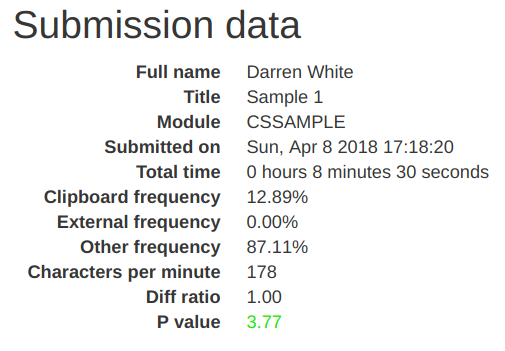
\includegraphics[height=.5\textheight,
    keepaspectratio=true,
    width=.5\textwidth,
    ]{figures/14-web-view-good-submission-data.png}
  }
  \caption[Submission Results A Data]{Example A submission data}
  \label{fig:results-a-submission-data}
\end{figure}

\newpage

\autoref{fig:results-a-submission-chart} shows the frequency of each source change over the time of development. There are several substantial changes which are noticeable immediately. Two clipboard changes occur just after 7 minutes, but notice that there were deletions of similar sizes just before these. This could potentially just be using copy/paste to move a piece of code. Similarly with the last two large changes, these could be part of a large refactoring method or reformatting. These changes can be individually looked at in detail in the \textit{large changes} below the chart.

\begin{figure}[H]
  \centering
  \fbox{
    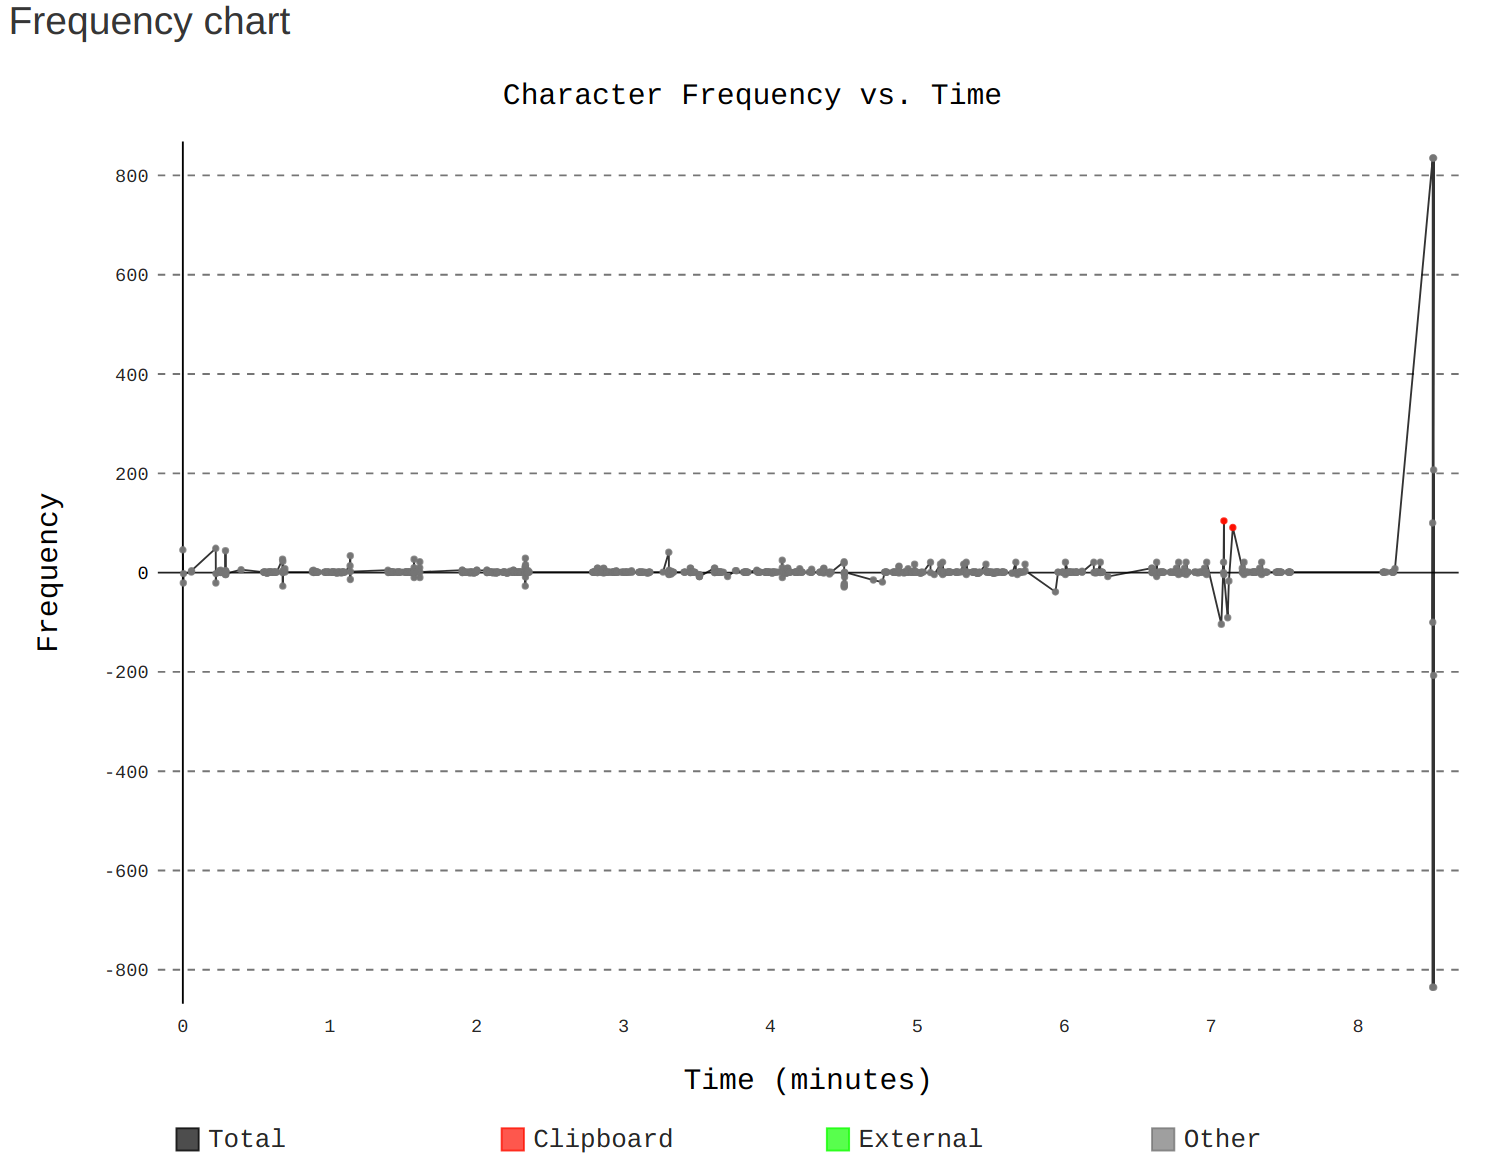
\includegraphics[height=\textheight,
    keepaspectratio=true,
    width=\textwidth,
    ]{figures/15-web-view-good-submission-chart.png}
  }
  \caption[Submission Results A Chart]{Example A submission FTS chart. Useful for identifying large changes.}
  \label{fig:results-a-submission-chart}
\end{figure}

\newpage

\autoref{tbl:results-a-submission-changes} shows the large changes for this example submission. The size of a large change was defined as 91 in this case (the default is 200). This can be changed by setting the \texttt{large\_change\_size} URL GET parameter. The content in the \textbf{OldString} and \textbf{NewString} columns have been replaced with letters. The content is not particularly interesting in this case. Note that each letter used denotes a unique piece of code. For example, all cells with \textit{A} represent the same piece of code.

Let's start with the first two rows. Row 0 shows us that \textit{A} was removed and in row 1 it was pasted in a different location. As the \textbf{NewString} cell of row 0 is empty we can identify that it was removed. We know \textit{A} was then pasted in a different location due to the row 1 \textbf{Source} being CLIPBOARD and the row 1 \textbf{Offset} being different to that of row 0. Also note that the time difference between rows 0 and 1 is around 1 second. The same scenario occurs for rows 2 and 3.

The next four pairs of rows, all share a similar scenario too. Firstly, the time difference between each pair is approximately 1ms. This indicates that this is most likely from an automatic refactoring or reformatting process. We can also see that the \textbf{NewString} content is immediately removed from another location showing that it was most likely moved.

After analysing the metrics, FTS chart, and large changes, this submission seems to have no identifiable acts of plagiarism.

\begin{table}[H]
\begin{center}
\begin{tabular}{|r|l|r|l|r|r|l|l|}
\hline
\textbf{Id} & \textbf{Path} & \multicolumn{1}{l|}{\textbf{Timestamp}} & \textbf{Source} & \multicolumn{1}{l|}{\textbf{Size}} & \multicolumn{1}{l|}{\textbf{Offset}} & \textbf{OldString} & \textbf{NewString} \\ \hline
0 & src/BingoCaller.java & 7.069433 & OTHER & 104 & 825 & \textit{A} &  \\ \hline
1 & src/BingoCaller.java & 7.087116 & CLIPBOARD & 104 & 717 &  & \textit{A} \\ \hline
2 & src/BingoCaller.java & 7.112766 & OTHER & 91 & 605 & \textit{B} &  \\ \hline
3 & src/BingoCaller.java & 7.147666 & CLIPBOARD & 91 & 838 &  & \textit{B} \\ \hline
4 & src/BingoCaller.java & 8.508266 & OTHER & 835 & 1090 &  & \textit{C} \\ \hline
5 & src/BingoCaller.java & 8.508283 & OTHER & 835 & 254 & \textit{C} &  \\ \hline
6 & src/BingoCaller.java & 8.508283 & OTHER & 100 & 254 &  & \textit{D} \\ \hline
7 & src/BingoCaller.java & 8.508300 & OTHER & 100 & 1190 & \textit{D} &  \\ \hline
8 & src/BingoCaller.java & 8.514716 & OTHER & 835 & 1191 &  & \textit{E} \\ \hline
9 & src/BingoCaller.java & 8.514733 & OTHER & 835 & 355 & \textit{E} &  \\ \hline
10 & src/BingoCaller.java & 8.514733 & OTHER & 207 & 355 &  & \textit{F} \\ \hline
11 & src/BingoCaller.java & 8.514750 & OTHER & 207 & 1398 & \textit{F} &  \\ \hline
\end{tabular}
\end{center}
\caption[Submission Results A Changes]{Example A submission large changes. Useful for identifying possible cases of plagiarism. \textit{Note: The code samples in the \textbf{Old String} and \textbf{New String} columns have been replaced with symbols. The content in these is not of particular use.}}
\label{tbl:results-a-submission-changes}
\end{table}

\newpage

\section{Example B}
Similar to Example A, we will look at the submission data, FTS chart, and large changes. \autoref{fig:results-b-submission-data} already shows a major red flag with the \textbf{P value} being 134.15. Looking more closely at the other values, it is easy to see why the \textbf{P value} is so high. 90.55\% of the code was copy/paste and it was completed in 19 seconds. The FTS chart shown in \autoref{fig:results-b-submission-chart} also backs this up. The chart shows a massive spike where code was pasted. The chart also shows that no code was deleted from the project at all.

\begin{figure}[H]
  \centering
  \fbox{
    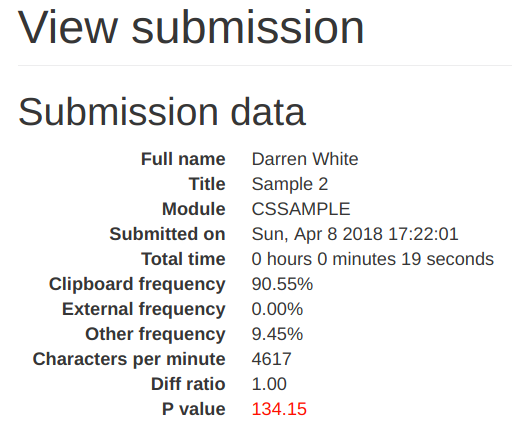
\includegraphics[height=.4\textheight,
    keepaspectratio=true,
    width=.4\textwidth,
    ]{figures/11-web-view-bad-submission-data.png}
  }
  \caption[Submission Results B Data]{Example B submission metrics}
  \label{fig:results-b-submission-data}
\end{figure}

\begin{figure}[H]
  \centering
  \fbox{
    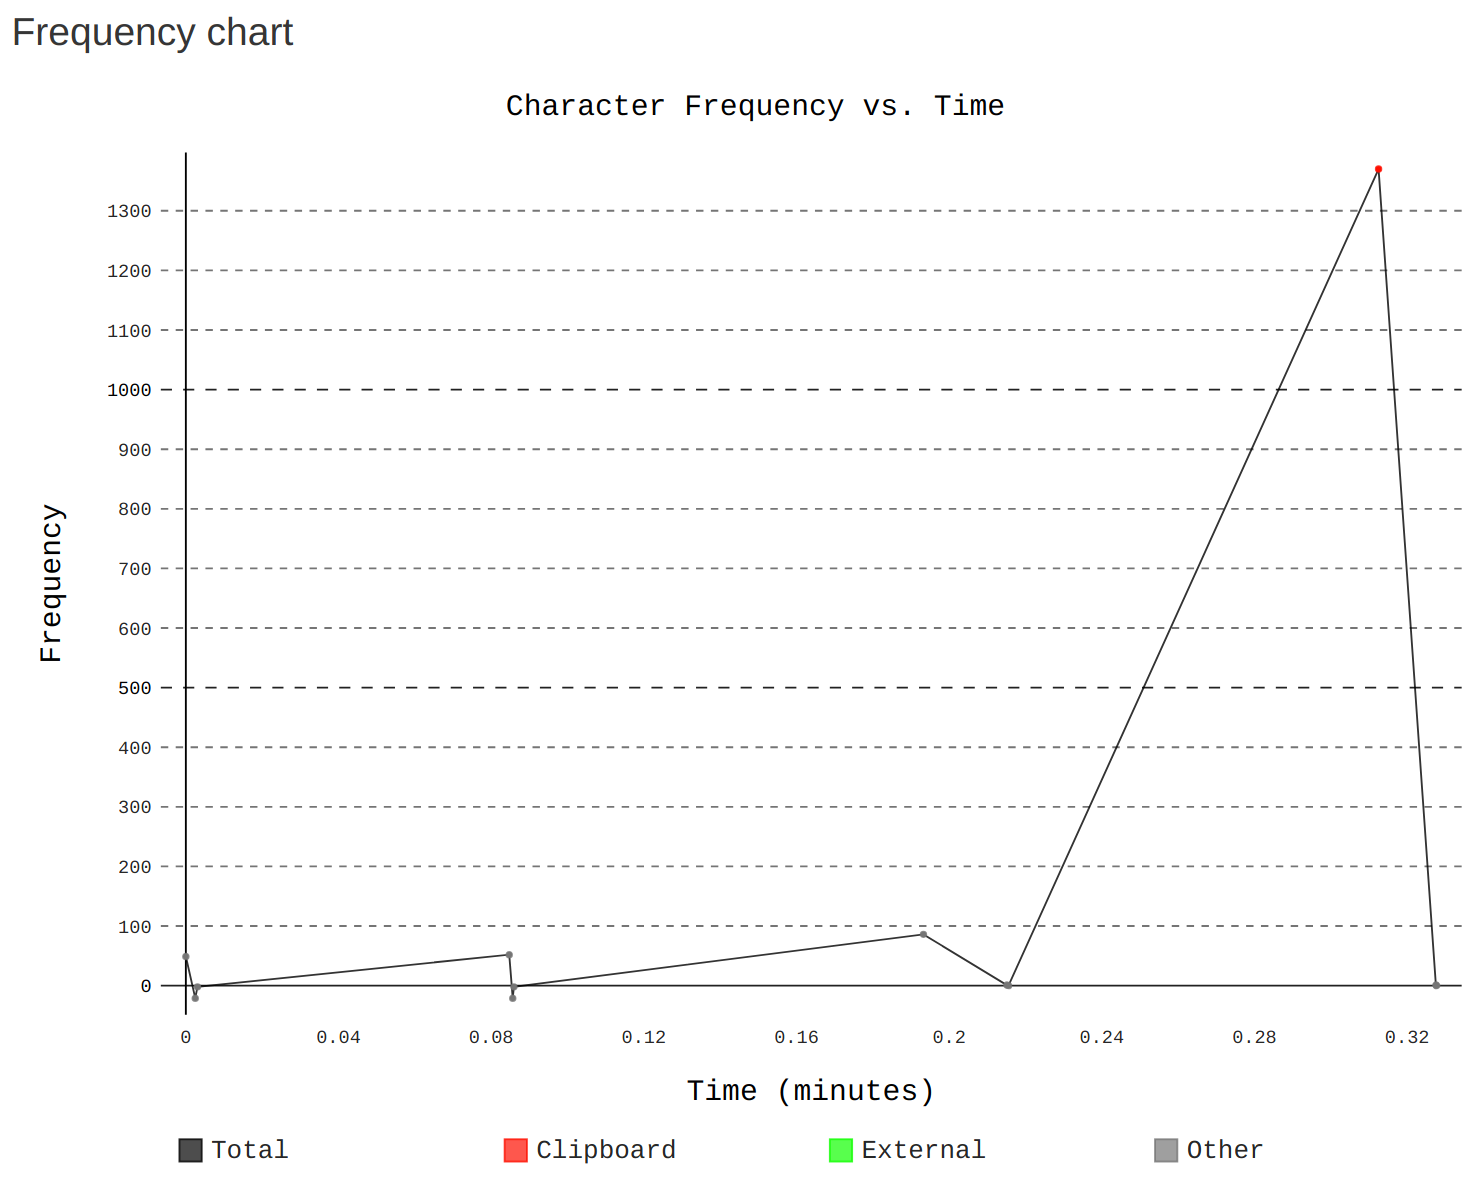
\includegraphics[height=.8\textheight,
    keepaspectratio=true,
    width=.8\textwidth,
    ]{figures/12-web-view-bad-submission-chart.png}
  }
  \caption[Submission Results B Chart]{Example B submission FTS chart. Useful for identifying large changes.}
  \label{fig:results-b-submission-chart}
\end{figure}

Below the \textbf{Old String} and \textbf{New String} values are shown for the CLIPBOARD change. \autoref{cde:old-string} shows the original file with an empty public class statement. In \autoref{cde:new-string} the pasted contents are displayed. The bulk of the pasted contents are not displayed as it is not valuable to this analysis. However, the pasted contents accounts for 90\% of the project and completes the file. This provides clear evidence of plagiarism.

%TC:ignore
\begin{code}
\begin{minted}[breaklines,
               linenos,
               frame=lines]{java}
public class BingoCaller {
}
\end{minted}
\caption[Submission Results B Old String]{Example B Change Old String}
\label{cde:old-string}
\end{code}
%TC:endignore

%TC:ignore
\begin{code}
\begin{minted}[breaklines,
               linenos,
               frame=lines]{java}
import java.security.SecureRandom;
import java.util.*;

public class BingoCaller {

    // Lots of copy and pasted code here
    // Removed it as it is unnecessary
    
}
\end{minted}
\caption[Submission Results B New String]{Example B Change New String}
\label{cde:new-string}
\end{code}
%TC:endignore
